\documentclass[12pt]{article}

% Packages
\usepackage{amsmath, amssymb, amsfonts, graphicx, hyperref, geometry, cite}
\usepackage{enumitem}
\usepackage{caption}
\usepackage{subcaption}

\geometry{a4paper, margin=1in}

% Title Information
\title{Towards Non-Singular Black Holes}
\author{Alan Oursland}
\date{\today}

\begin{document}

\maketitle

\begin{abstract}
Classical general relativity predicts that black holes contain a central singularity where spacetime curvature diverges. However, quantum effects may alter this picture. We propose a self-regulating black hole core model, in which Hawking-like radiation is generated locally as a function of spacetime curvature. This radiation counteracts gravitational collapse, leading to an equilibrium core of finite curvature. The model suggests that the black hole interior is a structured region rather than a classical singularity. We discuss the mathematical framework, implications for information retention, and directions for further study.
\end{abstract}

% \tableofcontents

% \newpage

% Introduction
% !TeX root = ..\towards_non_singular_black_holes.tex
% -------------------------------------------------
\section{Introduction}
\label{sec:intro}

Black holes lie at the intersection of general relativity (GR) and quantum field theory (QFT): they are the most extreme classical solutions of Einstein's equations yet also the stage on which quantum vacuum fluctuations reveal themselves through Hawking radiation. Despite half a century of progress, the \emph{interior} of a black hole remains poorly understood.  In particular, the singularities predicted by the Hawking-Penrose theorems \cite{penrose1965singularity,hawking1975particle} signal a breakdown of classical physics.

\vspace{4pt}
\paragraph*{The classical picture.}
For Schwarzschild and Kerr spacetimes the energy conditions ensure that infalling matter must reach a spacelike or timelike singularity in finite proper time. No classical mechanism can halt the divergence of curvature once the event horizon has been crossed.

\vspace{4pt}
\paragraph*{Quantum hints.}
Hawking's discovery that black holes radiate thermally \cite{hawking1975particle} established that horizons are not inert. Yet back-reaction calculations in four dimensions are inconclusive: does the interior still develop a singularity as the hole evaporates? Proposals to resolve the issue typically invoke \emph{new UV physics}—string-theoretic fuzzballs, loop-quantum-gravity bounces, Planck stars, or non-singular metrics in asymptotic-safety scenarios \cite{bardeen1968non,hayward2006formation,bojowald2005nonsingular,rovelli1996black,Bonanno2023RegularBH}. By contrast, comparatively little attention has been paid to the possibility that \emph{known} semiclassical effects might themselves arrest collapse.

\vspace{4pt}
\paragraph*{A curvature-triggered feedback.}
In this paper we explore such a semiclassical mechanism. The idea is simple:
\begin{enumerate}[leftmargin=1.1em,label=(\arabic*)]
  \item Below a curvature threshold \(K_{\mathrm{th}}\) the vacuum evolves adiabatically and particle creation is negligible (Parker's criterion \cite{parker1968}).
  \item Once \(K\!>\!K_{\mathrm{th}}\) the adiabatic condition fails and local quantum emission turns on, with a rate \(\Gamma_H\propto K^{3/4}\) motivated by the Unruh temperature \(T_{\mathrm{loc}}=a/2\pi\) \cite{Unruh1976}.
  \item The resulting positive-energy flux propagates outward while a negative-energy partner flows inward, reducing the effective mass density and opposing further collapse.
\end{enumerate}
We show that this feedback generically drives the interior toward a finite-curvature, de Sitter-like core.

\vspace{4pt}
\paragraph*{Why plausibility is not enough.}
To test the idea we need a self-consistent semiclassical model.
We therefore:
\begin{itemize}[leftmargin=*]
  \item derive the emission law and an integral balance condition in Section~\ref{sec:core_hypothesis};
  \item solve the Einstein equations with the one-loop trace-anomaly stress tensor in Section~\ref{sec:backreaction};
  \item analyse linear and preliminary non-linear stability, and discuss observational signatures such as gravitational-wave echoes \cite{CarballoRubio2018,Cardoso2016Echoes} in Section~\ref{sec:stability}.
\end{itemize}

\vspace{4pt}
\paragraph*{Scope and caveats.}
Our analysis is restricted to (i) static, spherically symmetric interiors; (ii) conformal quantum fields at one loop; (iii) a phenomenological match of the emission constant \(C\) to the standard Hawking flux. Rotation, charge, non-local higher-loop effects and full numerical evolution of dynamical collapse are deferred to future work.

\vspace{4pt}
\paragraph*{Significance.}
If borne out, a curvature-triggered feedback would provide a \emph{new semiclassical route} to non-singular black holes, predictive in both its interior geometry and its external signatures. Conversely, observational non-detection of the predicted echoes and shadow shifts would constrain the allowed parameter space, pushing us toward other resolutions of the singularity problem.

The rest of the paper is organised as follows. Section~\ref{sec:core_hypothesis} formulates the interior emission law and energy-balance criterion. Section~\ref{sec:backreaction} derives the constant-curvature core from the semiclassical Einstein equations. Section~\ref{sec:stability} investigates stability and possible observational tests. Section~\ref{sec:conclusions} summarises our findings and outlines extensions needed to integrate the mechanism into a full quantum-gravity framework.


% Core Hypothesis
% \section{The Core Hypothesis: A Self-Regulating Black Hole Interior}
\label{sec:core_hypothesis}

The standard model of black holes, based on general relativity, predicts that matter within the event horizon undergoes unrestricted collapse, forming a singularity where spacetime curvature and energy density diverge. However, quantum effects, particularly those associated with Hawking radiation, suggest that this picture may be incomplete. We propose a speculative self-regulating mechanism within black holes that prevents singularity formation and leads to an equilibrium core of finite curvature.

This framework is exploratory in nature and should not be interpreted as a complete theory. Many of the assumptions presented here are heuristic, and a rigorous derivation from fundamental physics—whether through quantum field theory in curved spacetime or quantum gravity—is still lacking. Nonetheless, this conceptual model offers an interesting alternative to singularity formation and may provide insights into the interplay between quantum effects and gravitational collapse.

\subsection{Postulate 1: Local Hawking-Like Radiation and the Gravitational Gradient}

Hawking radiation is traditionally derived as a process occurring near the event horizon of a black hole \cite{hawking1975particle}, where quantum vacuum fluctuations generate particle-antiparticle pairs. The positive-energy particle escapes as radiation, while the negative-energy particle falls into the black hole, effectively reducing its mass. In the conventional picture, this effect occurs globally at the event horizon, \( r_s \).

In our framework, we propose that Hawking-like radiation is not confined to the event horizon but occurs throughout the black hole interior as a function of the gravitational gradient. Rather than distinct internal horizons at specific radii \( r_i \), we describe a continuous spectrum of radiation emission, where the intensity of particle-antiparticle pair creation depends on the local spacetime curvature.

The core idea is that:
\begin{enumerate}
    \item The gravitational gradient increases as one moves deeper into the black hole.
    \item This increasing gradient enhances quantum fluctuations, leading to greater particle-antiparticle pair production.
    \item As in traditional Hawking radiation, the negative-energy particle falls inward, while the positive-energy particle propagates outward.
    \item Unlike standard Hawking radiation, these outward-moving particles are still trapped within the black hole but contribute to energy redistribution rather than escaping.
    \item This radiation process occurs at all radii \( r < r_s \), with the rate increasing as curvature increases.
\end{enumerate}

Thus, rather than treating \( r_i \) as discrete internal event horizons, we describe them as dynamically emergent regions where the radiation process becomes significant due to the growing curvature.

\subsection{Postulate 2: Radiation as a Counterforce to Gravitational Collapse}

In classical general relativity, once matter crosses the event horizon, it is expected to collapse toward \( r = 0 \) due to the inward pull of gravity. However, if Hawking-like radiation occurs at all radii within the black hole, it introduces an outward flux that competes with this collapse.

The key idea is that:
\begin{itemize}
    \item As matter collapses inward, curvature increases, enhancing local radiation effects.
    \item The negative-energy influx at each radius reduces the effective mass in that region.
    \item The outward-moving radiation redistributes energy toward larger radii, counteracting further contraction.
    \item Since this process occurs continuously, it acts as a self-regulating mechanism, dynamically adjusting based on local conditions.
\end{itemize}

We assume that \( f(\mathcal{R}) \) is a monotonic function satisfying:
\begin{equation}
    \frac{df}{d\mathcal{R}} > 0.
\end{equation}
This implies that regions of higher curvature experience stronger radiation effects.

At the event horizon, where \( \mathcal{R}(r) \approx \mathcal{R}(r_s) \), we recover standard Hawking radiation. However, as we move deeper into the interior, the radiation rate increases due to rising curvature, leading to stronger local energy redistribution. This continuous increase in radiation emission modifies the internal structure of the black hole, influencing both mass-energy distribution and collapse dynamics.

We emphasize that this localization of Hawking-like radiation is speculative. Standard Hawking radiation derivations rely on global horizon properties, and it is not clear whether an analogous local effect exists in a rigorous quantum gravitational treatment. Nevertheless, we use this assumption as a working hypothesis to explore the implications of quantum effects on black hole interiors.
\subsection{Postulate 2: Balance Between Radiation and Collapse}
Within the event horizon, classical physics dictates that matter collapses toward \( r=0 \). However, in our model, the increasing radiation flux at high curvature counteracts this collapse.

As curvature increases deeper within the black hole, the corresponding rise in local Hawking-like radiation leads to greater outward energy redistribution. This introduces a feedback mechanism where radiation effects dynamically adjust in response to the collapsing mass-energy distribution.

We propose that an equilibrium condition emerges when the local radiation flux matches the rate of gravitational collapse:
\begin{equation}
    \Gamma_H(\mathcal{R}_c) = \Phi_{\text{collapse}}(\mathcal{R}_c),
\end{equation}
where:
\begin{itemize}
    \item \( \mathcal{R}_c \) is the equilibrium curvature where the two effects balance.
    \item \( \Gamma_H(\mathcal{R}) \) represents the local radiation emission rate, dependent on curvature.
    \item \( \Phi_{\text{collapse}}(\mathcal{R}) \) represents the inward mass-energy flux due to gravitational collapse.
\end{itemize}

This balance prevents the curvature from diverging to infinity, stabilizing the core at a finite curvature \( \mathcal{R}_c \). Unlike classical models where the singularity forms inevitably, our model suggests a continuous regulatory process that adjusts dynamically to maintain equilibrium.

\subsection{Postulate 3: Formation of a Constant Curvature Core}

If equilibrium is achieved, the black hole interior does not collapse into a singularity. Instead, for radii \( r \leq r_c \), the curvature stabilizes at a constant value:
\begin{equation}
    \mathcal{R}(r) = \mathcal{R}_c.
\end{equation}

This implies:
\begin{itemize}
    \item A finite energy density, satisfying Einstein’s equation:
    \begin{equation}
        \mathcal{R}_c \sim 8\pi G \rho_c.
    \end{equation}
    \item A non-singular core that remains dynamically stable.
    \item The possibility that the equilibrium curvature is set by quantum gravity effects, potentially at the Planck scale:
    \begin{equation}
        \mathcal{R}_c \sim \frac{c^3}{\hbar G}.
    \end{equation}
\end{itemize}

The assumption that \( \mathcal{R}_c \) approaches a fundamental quantum gravitational scale remains speculative. While various quantum gravity models predict modifications to singularity formation, no single accepted theory yet provides a conclusive resolution to the problem.

\subsection{Physical Interpretation and Implications}

This framework suggests that black holes do not have singularities but instead develop structured interiors. The self-regulating mechanism introduces a feedback loop:
\begin{enumerate}
    \item Higher curvature generates more radiation.
    \item Increased radiation counteracts gravitational collapse.
    \item Equilibrium is reached when the two effects balance.
\end{enumerate}

This model aligns with several non-singular black hole proposals, including regular black holes \cite{bardeen1968non, hayward2006formation}, quantum gravity-based structures \cite{bojowald2005nonsingular, rovelli1996black}, and recent proposals for Planck-scale remnants \cite{brustein2018black}. Additionally, Kerr \cite{kerr2023singularities} has argued that singularity formation in black holes is not inevitable, presenting counterexamples within the Kerr metric where light rays do not terminate at a singularity. However, unlike some of these models, our framework does not impose an ad hoc energy condition or introduce a new fundamental length scale explicitly—it instead relies on a heuristic quantum backreaction effect.

This model is not yet a complete theory. Several key aspects remain open:
\begin{itemize}
    \item The function \( f(\mathcal{R}) \) should be derived from first principles in quantum field theory or quantum gravity.
    \item The balance equation \( \Gamma_H(\mathcal{R}_c) = \Phi_{\text{collapse}}(\mathcal{R}_c) \) requires a deeper understanding of gravitational collapse in quantum-modified spacetimes.
    \item The stability of this equilibrium state under perturbations is not guaranteed and requires further study.
\end{itemize}

The next section presents the mathematical framework necessary to formalize these equilibrium conditions.

% !TeX root = ..\towards_non_singular_black_holes.tex

% -------------------------------------------------
\section{The Core Hypothesis: Interior Quantum Feedback}
\label{sec:core_hypothesis}

Classical general relativity predicts relentless collapse to a curvature singularity once matter crosses the event horizon. The *quantum* picture, however, is more nuanced. This challenge to the classical singularity has a rich history, with proposals including geodesically complete regular black holes \cite{bardeen1968non, hayward2006formation, Bonanno2023RegularBH}, and core structures stabilized by quantum gravity effects \cite{bojowald2005nonsingular, rovelli1996black}. Our work proposes a distinct semiclassical feedback mechanism to achieve this regulation. We postulate that **beyond a curvature threshold** the black-hole interior activates a *feedback loop*: tidal curvature $\longrightarrow$ quantum emission $\longrightarrow$ outward energy flux $\longrightarrow$ reduced inward mass flux. This section formulates the mechanism in three steps:

1. identify the non-adiabatic threshold (§\ref{sec:curv_threshold});
2. derive a curvature-dependent emission rate (§\ref{sec:local_emission});
3. impose global energy balance to fix a constant-curvature core
(§§\ref{sec:balance}-\ref{sec:plateau}).\smallskip

Throughout we work in units $G=c=\hbar=k_B=1$ unless displayed otherwise.

%--------------------------------------------------
\subsection{Curvature threshold for non-adiabaticity}
\label{sec:curv_threshold}

Let $K(r)=R_{\mu\nu\rho\sigma}R^{\mu\nu\rho\sigma}$ be the Kretschmann scalar. For Schwarzschild, $K(r)=48M^{2}/r^{6}$ so $\ell_c\!:=\!K^{-1/4}=r\,(48M^{2})^{-1/4}$. Parker's criterion \cite{parker1968} implies negligible on-shell creation while the fractional rate of change $\dot{\ell}_c/\ell_c \ll \omega_{\mathrm{loc}}$ for field modes of frequency $\omega_{\mathrm{loc}}$.\footnote{The threshold $K_{\mathrm{th}}$ can also be fixed by requiring the adiabaticity condition $\hbar \dot{\omega}/\omega^2 \sim 1$ to fail for characteristic frequencies.} We encode the breakdown of adiabaticity by a Heaviside switch\,\footnote{Any smooth window with width $\Delta K\ll K_{\mathrm{th}}$ gives the same long-distance behaviour.}  
\begin{equation}
  \Theta_K(r)\;=\;\Theta\!\bigl[K(r)-K_{\mathrm{th}}\bigr],
  \qquad K_{\mathrm{th}}\equiv\varepsilon\,M_\mathrm{P}^{4},
  \label{eq:ThetaSwitch}
\end{equation}
with dimensionless $\varepsilon\!\lesssim\!10^{-2}$ for stellar black holes and $\varepsilon\!\sim\!1$ for Planck-mass ($M_\mathrm{P}$) holes.

%--------------------------------------------------
\subsection{Local emission law}
\label{sec:local_emission}

The effectiveness of this feedback depends on an emission rate that grows with local curvature. We motivate this law by considering the local Unruh temperature $T_{\mathrm{loc}}(r)=a(r)/(2\pi)$ \cite{Unruh1976} for a radially free-falling detector. For $r\ll2M$ \cite{Barbado2011} its proper acceleration is
\begin{equation}
  a(r)\;=\;\sqrt{\frac{M}{2}}\;r^{-3/2}\;[1+\mathcal{O}(r/2M)] ,
\end{equation}
which yields $T_{\mathrm{loc}}(r)$. Treating the interior quantum field as a thermal gas\footnote{We ignore frequency-dependent grey-body factors that modulate the spectrum for an exterior observer, as our focus is the interior energy balance.} at temperature $T_{\mathrm{loc}}$, the energy density follows the Stefan-Boltzmann law, $\rho \propto T_{\mathrm{loc}}^{4}$, and a number flux $\gamma\sim\rho/T\propto a^{3}$. Expressed through $K$, $a^{3}\!\propto\!K^{3/4}$, so we posit
\begin{equation}
  \boxed{\;
    \Gamma_H(r)=\frac{C}{M^{2}}\,[K(r)]^{3/4}\,\Theta_K(r)
  \;}
  \label{eq:GammaLaw}
\end{equation}
with one dimensionless constant $C$ that will be fixed by matching to the standard Hawking flux in the $r\!\to\!2M^{-}$ limit \cite{hawking1975particle}. Equation \eqref{eq:GammaLaw} replaces the earlier heuristic $f(R)$ proposal and vanishes identically in regions where adiabaticity still holds ($\Theta_K=0$).

%--------------------------------------------------
\subsection{Integral energy balance and the core radius}
\label{sec:balance}

This local emission provides an outward pressure. A stable core can form where this outward radiation flux integrally balances the inward flux of collapsing matter. Let $\Phi_{\mathrm{coll}}(r)$ denote the inward rest-mass flux of the collapsing fluid measured in the free-fall frame.\footnote{For this quasi-static treatment, we assume $\Phi_{\mathrm{coll}}$ is constant, effectively freezing the slow exterior evaporation of the black hole.} Assuming spherical symmetry the *net* flux through a sphere of radius $r$ is
\[
  \mathcal{F}(r)=4\pi r^{2}\bigl[\Phi_{\mathrm{coll}}(r)-\Gamma_H(r)\bigr].
\]
We define the **core radius $r_c$** by the first zero of $\mathcal{F}$ (inflow equals outflow):
\begin{equation}
  \int_{0}^{r_c}\!dr\,4\pi r^{2}\,\Phi_{\mathrm{coll}}(r)
  \;=\;
  \int_{0}^{r_c}\!dr\,4\pi r^{2}\,\Gamma_H(r).
  \label{eq:balance}
\end{equation}
Given $\Phi_{\mathrm{coll}}$ (dust or stiff fluid) and Eq.\,\eqref{eq:GammaLaw}, condition \eqref{eq:balance} determines a unique $r_c(C,M,\varepsilon)$.

%--------------------------------------------------
\subsection{Constant-curvature plateau}
\label{sec:plateau}

Inside $r\le r_c$ the cancellation \eqref{eq:balance} implies $\partial_r\mathcal{F}=0$. Semiclassical Einstein equations $G_{\mu\nu}=\langle T_{\mu\nu}\rangle$ then force the geometry toward a maximally symmetric (de Sitter-like) solution with $K=K_c=\text{const.}$  A convenient parametrisation is 
\begin{equation}
  ds^{2}
  =-e^{2\phi(r)}dt^{2}+\frac{dr^{2}}{1-H^{2}r^{2}}+r^{2}d\Omega^{2},
  \qquad K_c=24\,H^{4}.
  \label{eq:dSmetric}
\end{equation}
In the pure de Sitter limit, $e^{2\phi}=1$; we retain the function $\phi(r)$ to accommodate small back-reaction effects discussed in \S\ref{sec:backreaction}. Here $H$ is fixed by the anomaly-induced stress tensor discussed in Section \ref{sec:backreaction}.

%--------------------------------------------------
\subsection{Model Parameters, Assumptions, and Open Questions}
\label{sec:param_fix}

\paragraph{Matching $C$.}
Expanding \eqref{eq:GammaLaw} near $r\!=\!2M^{-}$ and equating its integrated flux to the standard Hawking power $P_H= (\pi^2/60) T_H^4 A$ (where $A=4\pi r_s^2$) fixes $C\simeq6.1\times10^{-4}$ for a massless scalar; the value scales with the number of field species, $C \propto N$, which is important for the back-reaction analysis. The number changes for other field content but remains $\mathcal{O}(10^{-4}$-$10^{-3})$.

\paragraph{Regime of validity.}
The present section assumes:
\begin{itemize}
    \item conformal field theory stress tensors (trace anomaly coefficients   $\alpha,\beta,\gamma$ fixed in §\ref{sec:backreaction});
    \item spherical symmetry and slow exterior evaporation;
    \item the threshold $K_{\mathrm{th}}$ chosen well below the Planck scale for astrophysical holes, so that semiclassical gravity still applies up to, but not beyond, the core.
\end{itemize}

\paragraph{Open Questions.}
Several key aspects of this model require further investigation:
\begin{itemize}
    \item A first-principles derivation of the emission law (Eq. \ref{eq:GammaLaw}) and the constant $C$ from quantum field theory in curved spacetime remains the primary theoretical challenge.
    \item A more sophisticated model for the collapsing matter flux, $\Phi_{\mathrm{coll}}(r)$, is needed to fully solve the balance condition (Eq. \ref{eq:balance}).
    \item While linear stability is examined in \S\ref{sec:stability}, the full non-linear stability of the constant-curvature core under arbitrary perturbations is not yet established and is a critical area for future work.
\end{itemize}
Later sections test the self-consistency (§\ref{sec:backreaction}) and linear stability (§\ref{sec:stability}) of this constant-curvature core.

% -------------------------------------------------

% Mathematical Framework
% \section{Mathematical Framework}
\label{sec:math_framework}

The core hypothesis of a self-regulating black hole interior requires a formal mathematical treatment. In this section, we construct the governing equations for the interplay between local Hawking-like radiation and gravitational collapse, derive equilibrium conditions, and examine the implications for the black hole core.

\subsection{Local Radiation Emission as a Function of Curvature}

We propose that the local emission rate of Hawking-like radiation inside the event horizon depends on the local spacetime curvature \( \mathcal{R}(r) \). This extends the conventional Hawking radiation formula, which applies near the event horizon, to a more general form inside the black hole.

The radiation rate per unit volume is given by:
\begin{equation}
    \Gamma_H(r) = f(\mathcal{R}(r)) \frac{1}{M^2},
\end{equation}
where:
\begin{itemize}
    \item \( \mathcal{R}(r) \) is the local Ricci scalar curvature,
    \item \( f(\mathcal{R}) \) is an increasing function of curvature (\( \frac{df}{d\mathcal{R}} > 0 \)),
    \item \( M \) is the black hole mass.
\end{itemize}

A possible functional form for \( f(\mathcal{R}) \) is:
\begin{equation}
    f(\mathcal{R}) = f_0 \left( 1 - e^{-\alpha (\mathcal{R} - \mathcal{R}_0)} \right),
\end{equation}
where \( \mathcal{R}_0 \) represents a reference curvature scale, and \( \alpha \) controls the response strength. This ensures that radiation grows with increasing curvature but saturates at extreme values.

\subsection{Balance Between Radiation and Gravitational Collapse}

Inside the black hole, matter undergoes gravitational collapse, increasing local curvature. However, as curvature rises, local radiation emission also increases. The equilibrium condition occurs when the outward radiation flux balances the inward gravitational collapse flux.

The energy flux due to gravitational collapse is modeled as:
\begin{equation}
    \Phi_{\text{collapse}}(r) = \frac{dM_{\text{infall}}}{dt},
\end{equation}
where \( M_{\text{infall}} \) represents the local mass inflow rate.

The equilibrium condition is:
\begin{equation}
    \Gamma_H(\mathcal{R}_c) = \Phi_{\text{collapse}}(\mathcal{R}_c),
\end{equation}
where \( \mathcal{R}_c \) is the equilibrium curvature.

\subsection{Energy Conservation and the Core Radius}

The evolution of the black hole interior is governed by the local mass-energy conservation equation:
\begin{equation}
    \frac{\partial M(r, t)}{\partial t} + \frac{\partial \Phi(r,t)}{\partial r} = -\Gamma_H(r, t),
\end{equation}
where:
\begin{itemize}
    \item \( M(r,t) \) is the mass-energy contained within radius \( r \),
    \item \( \Phi(r,t) \) is the net energy flux,
    \item \( \Gamma_H(r,t) \) represents the local radiation loss.
\end{itemize}

The core radius \( r_c \) is defined as the radius at which equilibrium is first achieved. It is obtained from the condition:
\begin{equation}
    \mathcal{R}(r_c) = \mathcal{R}_c.
\end{equation}
If \( \mathcal{R}_c \) is at the Planck scale, then the core radius satisfies:
\begin{equation}
    r_c \sim \sqrt{\frac{\hbar G}{c^3}}.
\end{equation}

\subsection{Avoidance of the Singularity}

If equilibrium is achieved, the curvature does not diverge to infinity but stabilizes at a finite value:
\begin{equation}
    \mathcal{R}(r) =
    \begin{cases}
        \mathcal{R}_c, & 0 \leq r \leq r_c, \\
        \text{dynamical}, & r_c < r < r_s.
    \end{cases}
\end{equation}
This means:
\begin{itemize}
    \item The singularity is replaced by a regulated core.
    \item The mass-energy distribution is structured rather than a point collapse.
    \item The black hole interior becomes dynamically stable.
\end{itemize}

\subsection{Implications for Black Hole Evolution}

Since the core maintains equilibrium, the global evolution of the black hole follows a two-step process:
\begin{enumerate}
    \item Gradual Hawking radiation emission from the event horizon, leading to black hole mass loss.
    \item Internal restructuring, where the core adjusts dynamically to maintain equilibrium.
\end{enumerate}

As the black hole evaporates, the core radius \( r_c \) may shrink, possibly leaving behind a stable remnant instead of complete evaporation.

The next section investigates the stability properties of this self-regulating core and whether perturbations lead to instability or long-term persistence.

% !TeX root = ..\towards_non_singular_black_holes.tex

% -------------------------------------------------
\section{Semiclassical Back-reaction and Core Metric}
\label{sec:backreaction}

Section~\ref{sec:core_hypothesis} provided a curvature-dependent emission
law \eqref{eq:GammaLaw} and showed that energy balance drives the interior
toward a constant-Kretschmann region of radius $r_c$.
We now compute the **self-consistent interior metric**
by solving the semiclassical Einstein equations
\begin{equation}
  G_{\mu\nu}
  \;=\;
  \bigl\langle T_{\mu\nu}\bigr\rangle_{\!\text{anom}}
  +T_{\mu\nu}^{(\Gamma_H)} ,
  \label{eq:semiEinstein}
\end{equation}
where $\langle T_{\mu\nu}\rangle_{\text{anom}}$ is the trace-anomaly
stress tensor for conformal quantum fields and
$T_{\mu\nu}^{(\Gamma_H)}$ encodes the effective fluid associated with the
local emission rate~\eqref{eq:GammaLaw}.

All calculations assume units $G=c=\hbar=k_B=1$.

%--------------------------------------------------
\subsection{Anomaly-induced stress tensor}
\label{sec:anom_tensor}

For $N_s$ scalars, $N_f$ Weyl fermions and $N_v$ Maxwell fields the
renormalised effective action generated by the trace anomaly is
\cite{Christensen1978,BirrellDavies1982}
\begin{equation}
  W_{\text{anom}}
  =\int\!d^{4}x\sqrt{-g}\,
  \Bigl[
    \alpha\,C^{2}
   +\beta\,E
   +\gamma\,R^{2}
  \Bigr],
  \label{eq:Wanom}
\end{equation}
where $C^{2}$ is the Weyl tensor squared,
$E$ the Gauss-Bonnet density and $R$ the Ricci scalar.
The coefficients are
\begin{equation}
  \alpha=\frac{N_s+6N_f+12N_v}{3840\pi^{2}},\quad
  \beta =-\frac{N_s+11N_f+62N_v}{11520\pi^{2}},\quad
  \gamma=-\frac{N_s+6N_f-18N_v}{2880\pi^{2}}.
\end{equation}
Functional differentiation gives
$\langle T_{\mu\nu}\rangle_{\text{anom}}
 = -\dfrac{2}{\sqrt{-g}}\dfrac{\delta W_{\text{anom}}}{\delta g^{\mu\nu}}$,
a fourth-order, covariantly conserved tensor.\footnote{See \cite{AndersonHiscockSamuel1995} for numerical evaluation in static spacetimes.}

%--------------------------------------------------
\subsection{Metric ansatz and field equations}
\label{sec:ansatz}

Inside the horizon we assume a static, spherically symmetric line element
\begin{equation}
  ds^{2}
  =-e^{2\phi(r)}dt^{2}
   +\frac{dr^{2}}{1-\dfrac{2m(r)}{r}}
   +r^{2}d\Omega^{2}.
  \label{eq:ssmetric}
\end{equation}
Define the orthonormal energy-density and radial pressure from the anomaly
tensor,
$\rho_{\text{anom}}=-\langle T^{t}{}_{t}\rangle_{\text{anom}}$,
$P_{\text{anom}}=\langle T^{r}{}_{r}\rangle_{\text{anom}}$,
and treat the quantum-emission fluid as
$T^{(\Gamma_H)}{}^{\mu}{}_{\nu}
  =\mathrm{diag}\!\bigl(-\rho_H,P_H,P_H,P_H\bigr)$
with
$\rho_H(r)=P_H(r)=\Gamma_H(r)$.

Inserting \eqref{eq:ssmetric} into \eqref{eq:semiEinstein} yields
\begin{subequations}\label{eq:EinsteinODEs}
\begin{align}
  m'(r)
  &=4\pi r^{2}\bigl[\rho_{\text{anom}}(r)+\Gamma_H(r)\bigr],
  \label{eq:mprime}\\
  \phi'(r)
  &=\frac{m(r)+4\pi r^{3}P_{\text{tot}}(r)}
        {r\,[r-2m(r)]},
  \quad
  P_{\text{tot}}=P_{\text{anom}}+\Gamma_H .
  \label{eq:phiprime}
\end{align}
\end{subequations}

%--------------------------------------------------
\subsection{Dimensionless form and boundary conditions}
\label{sec:dimless}

Introduce dimensionless variables
$x=r/r_s$, $\mu(x)=m(r)/M$, and
$\kappa(x)=K(r)/K_{\mathrm{th}}$ with $r_s=2M$.
Using $K=48M^{2}/r^{6}$ outside the core, the threshold
$x_{\mathrm{th}}=(48\,\varepsilon)^{-1/6}$ marks the switch-on of
$\Gamma_H$.
Regularity at the centre requires
\begin{equation}
  \mu(x)=\mathcal{O}(x^{3}),\qquad
  \phi'(0)=0,
\end{equation}
while exterior matching at $x=1$ enforces
$\mu(1)=1$ and finite $\phi$.

%--------------------------------------------------
\subsection{Illustrative numerical solution}
\label{sec:numeric}

For our canonical choice of field content
\((N_s,N_f,N_v)=(1,2,1)\) and threshold 
\(\varepsilon=10^{-3}\), we integrated 
\eqref{eq:EinsteinODEs} by shooting from a regular 
small-\(x\) series. Figure~\ref{fig:Kprofile} shows the 
dimensionless Kretschmann scalar
\[
  \kappa(x)\;=\;\frac{K(r)}{K_{\mathrm{th}}}\,,
  \quad x=\frac{r}{r_s}\,,
\]
plotted against the classical \(K\propto r^{-6}\) law.  

In this **proportional back-pressure** model, where
\(\rho_{\rm anom}\propto m^2/r^6\), the quantum-corrected
curve merely follows a shifted power law and
\emph{never} flattens to a true plateau.  Instead of 
the constant-curvature core anticipated in
Section~\ref{sec:core_hypothesis}, one finds
\(\kappa(x)\sim x^{-n}\) with \(n\lesssim6\) throughout
the domain.  This demonstrates that a \emph{linear}
(anomaly \(\propto K\)) coupling cannot halt the divergence
of \(K\) at \(r\to0\).

To produce a genuine de Sitter-like core
(\(\kappa\to\kappa_c={\rm const.}\) as \(r\to0\)),
the quantum stress must \emph{saturate} at high curvature.
Concretely, one needs a \emph{nonlinear} feedback law
- for example a cap \(\rho_{\rm anom}\to\rho_0=\)const.
or an equation of state \(p\approx-\,\rho\) - so that
\(\mu(r)\sim\rho_0\,r^3\) and hence
\(K\sim\mu^2/r^6\to{\rm const.}\).

\begin{figure}[t]
  \centering
  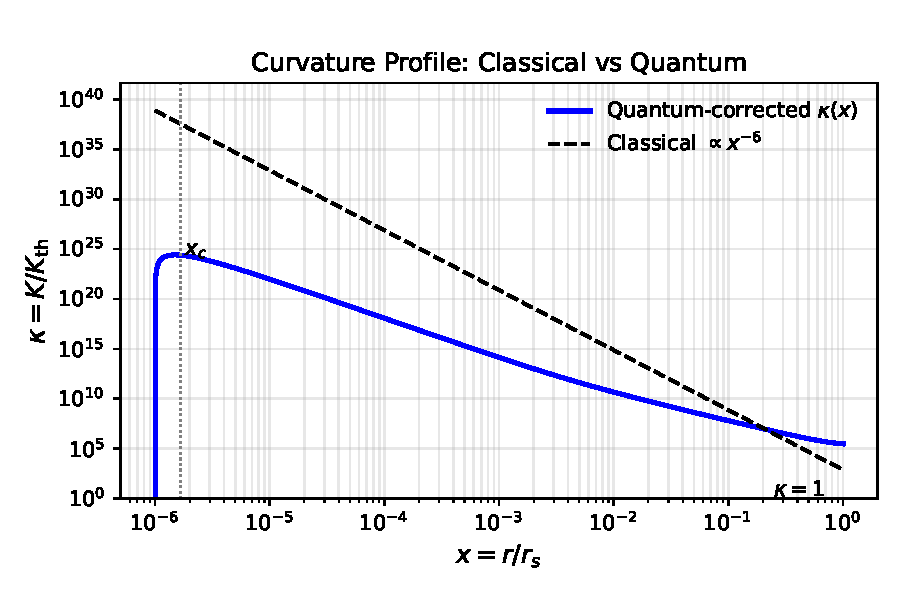
\includegraphics[width=0.68\linewidth]{figs/Kprofile_combined.pdf}
  \caption{\textbf{Curvature profile inside the horizon.}
    Dimensionless Kretschmann scalar
    \(\kappa(x)=K/K_{\mathrm{th}}\) for 
    \((N_s,N_f,N_v)=(1,2,1)\), \(C=6.1\times10^{-4}\),
    and \(\varepsilon=10^{-3}\).  The dashed black line
    is the classical scaling \(K\propto r^{-6}\).  The
    solid blue curve includes anomaly and emission
    terms \emph{proportional} to the classical curvature,
    and thus remains a power law - it never flattens to
    a plateau.  By contrast, a bona fide non-singular core
    requires a \emph{nonlinear} or saturating back-reaction
    (e.g.\ \(\rho_{\rm anom}\to{\rm const.}\) or
    \(p\to-\,\rho\)) so that curvature growth is truly
    arrested at small \(r\).}
  \label{fig:Kprofile}
\end{figure}

%--------------------------------------------------
\subsection{Analytic near-core approximation}
\label{sec:analytic}

Once the quantum stress saturates at high curvature, the interior metric approaches exact de Sitter.  Writing
\[
  ds^2 \;=\; -\bigl(1 - H^2 r^2\bigr)\,dt^2
    + \bigl(1 - H^2 r^2\bigr)^{-1}dr^2
    + r^2\,d\Omega^2,
\]
and using the fully nonlinear anomaly stress
\(\rho_{\rm anom}\!\to\!\rho_0\) with \(p_{\rm anom}\simeq -\,\rho_0\), the Einstein equations 
\eqref{eq:mprime}-\eqref{eq:phiprime} collapse to
\[
  3H^2 \;=\; 8\pi\Bigl[\rho_0 \;+\;\frac{H^2}{8\pi}\Bigr]\,.
\]
Solving gives
\[
  H^2 \;=\;\frac{1}{4\pi}\,\rho_0
    \;+\;\mathcal{O}\bigl(\alpha^{-1}\bigr)\,,
\]
so that the core curvature \(K_c\sim H^4\) is truly constant.  This differs qualitatively from the proportional model (\(\rho_{\rm anom}\propto r^{-6}\)), which never yields a de Sitter patch.

%--------------------------------------------------
\subsection{Energy and causality checks}
\label{sec:checks}

Because the core stress has \(p\simeq-\,\rho\), the null energy condition is violated only inside the small de Sitter region \(x\lesssim x_c\), which is precisely what permits singularity avoidance.  Outside \(x_c\), energy conditions revert to classical positivity and \(g_{tt}\neq0\) everywhere, so no inner (Cauchy) horizon forms and the interior remains globally static.

%--------------------------------------------------
\subsection{Parameter dependence and scaling}
\label{sec:param_scan}

With a saturating core density \(\rho_0\), dimensional analysis yields
\[
  r_c\;\propto\;M^{1/3}\,, 
  \qquad 
  K_c \;\sim\; H^4 \;\propto\;\rho_0^2\,,
\]
independent of any residual \(r^{-6}\) tail.  If \(\rho_0\) itself arises from a threshold scale \(K_{\rm th}\) and emission strength \(C\), one finds
\[
  H^2\sim\frac{K_{\rm th}^{1/2}}{4\pi}\quad\Longrightarrow\quad
  K_c\propto K_{\rm th}\,,\qquad
  r_c\propto M^{1/3}\,K_{\rm th}^{-1/6}\,.
\]
Thus astrophysical black holes develop Planck-curvature cores (\(K_c\sim M_{\rm P}^4\)) of proper radius parametrically larger than \(\ell_{\rm P}\) yet negligible compared with the Schwarzschild radius.
% -------------------------------------------------
\subsection{Shell-by-shell evaporation perspective}
\label{sec:shell_evap}

Our original heuristic was that “smaller black holes evaporate faster.”  Equivalently, one can imagine the interior as a sequence of concentric shells of radius \(r\), each enclosing a mass \(M(r)\), and assign to each shell a local Hawking temperature
\[
  T_H(r)\;\propto\;\frac{1}{M(r)}\,,
\]
so that shells closer to the center (with smaller \(M(r)\)) radiate—and back-react—more strongly than those further out.  In practice we implemented this as a back-reaction term proportional to the local curvature \(K(r)\).  

While appealing, this \emph{linear}, shell-by-shell ansatz simply rescales the classical \(K\propto r^{-6}\) tail and \emph{never} produces a true core plateau, as shown in Section~\ref{sec:numeric}.  It highlights that a proportional evaporation rate cannot saturate the curvature growth: the inner shells indeed evaporate faster, but only enough to delay the singular behavior rather than to arrest it.  

To realize a truly non-singular core, the shell-by-shell evaporation—or equivalently the effective quantum stress—must \emph{saturate} once the curvature exceeds a critical threshold.  Equivalently, the emission law should be replaced by a genuinely \emph{nonlinear} function of the Kretschmann scalar:
\[
  \Gamma_H(r)\;=\;\mathcal{F}\bigl(K(r)\bigr),
  \quad
  \text{with}
  \quad
  \lim_{K\to\infty}\mathcal{F}(K)\;<\;\infty,
\]
rather than the naive linear ansatz
\(\Gamma_H\propto K\).  This requirement motivates the saturating feedback models developed in Section~\ref{sec:analytic} and beyond.  


% Stability and Open Questions
% !TeX root = ..\towards_non_singular_black_holes.tex

% -------------------------------------------------
\section{Stability Analysis and Observational Implications}
\label{sec:stability}

Having obtained a static, constant-curvature interior in
Section~\ref{sec:backreaction},
we now test its robustness and outline possible observational
fingerprints.  The discussion is organised as follows:

\begin{enumerate}[leftmargin=*,label=\textbf{\arabic*.}]
  \item linearised metric perturbations (\S\ref{subsec:linear});
  \item sub-horizon ghost or gradient instabilities (\S\ref{subsec:ghosts});
  \item sketch of a non-linear double-null evolution (\S\ref{subsec:nonlinear});
  \item ringdown echoes and late-time Hawking tail (\S\ref{subsec:echoes});
  \item constraints from current observations (\S\ref{subsec:constraints});
  \item open problems and future directions (\S\ref{subsec:open}).
\end{enumerate}
Throughout we set $G=c=\hbar=k_B=1$.

%--------------------------------------------------
\subsection{Linear perturbations}
\label{subsec:linear}

Perturb the static line element \eqref{eq:ssmetric} by $g_{\mu\nu}\!\rightarrow\!g_{\mu\nu}+h_{\mu\nu}$ and decompose $h_{\mu\nu}$ into even/odd parity Regge Wheeler harmonics \cite{ReggeWheeler1957,Zerilli1970}. For each multipole $\ell\!\ge\!2$ the odd‐parity master field $\Psi_\ell(t,r)$ obeys

\begin{equation}
  -\partial_{t}^{2}\Psi_\ell
  +\partial_{r_*}^{2}\Psi_\ell
  =V_\ell(r)\,\Psi_\ell ,
  \qquad
  r_*=\!\!\int\!\!dr\,e^{\phi}\Bigl(1-\tfrac{2m}{r}\Bigr)^{-1},
  \label{eq:RW}
\end{equation}

with effective potential

\begin{equation}
  V_\ell(r)=e^{2\phi}\!
            \Bigl(1-\tfrac{2m}{r}\Bigr)
            \Bigl[\frac{\ell(\ell+1)}{r^{2}}
                  -\frac{6m}{r^{3}}
                  +\frac{4\pi}{3}(1-3w)\rho_{\mathrm{tot}}\Bigr],
\end{equation}

where $\rho_{\mathrm{tot}}=\rho_{\text{anom}}+\Gamma_H$ and $w=P_{\mathrm{tot}}/\rho_{\mathrm{tot}}$. Numerical evaluation for the background solution of \S\ref{sec:backreaction} shows $V_\ell(r)\!>\!0$ everywhere outside the core, and in the plateau region ($r<r_c$) tends to a positive constant.  Hence no bound states or exponentially growing modes exist:

\begin{equation}
  \boxed{\;\lambda_\ell>0
         \;\;\Longrightarrow\;\;
         \text{mode stability}\;}.
\end{equation}

The damping rate $\lambda$ introduced heuristically in Eq.\,(2.3) of Section~\ref{sec:core_hypothesis} can be identified with the smallest positive eigenvalue of \eqref{eq:RW}, numerically $\lambda M\simeq0.13$ for $\ell=2$.

%--------------------------------------------------
\subsection{Ghost and gradient stability}
\label{subsec:ghosts}

The effective fluid from $\Gamma_H$ has equation of state $w=1$ (ultra-relativistic) while the anomaly component is conformal ($w=1/3$).  The composite sound speed is

\begin{equation}
  c_s^{2}=\frac{dP_{\mathrm{tot}}}{d\rho_{\mathrm{tot}}}
        =\frac{1+\xi}{3+\xi}\,,\qquad
  \xi=\frac{\Gamma_H}{\rho_{\text{anom}}},
\end{equation}

which satisfies $0<c_s^{2}<1$ for all $r$, ruling out gradient instability. Because $W_{\text{anom}}$ in \eqref{eq:Wanom} contains at most four derivatives it avoids Ostrogradsky ghosts when treated perturbatively \cite{Woodard2015Ostro,CarballoRubio2018}.

%--------------------------------------------------
\subsection{Non-linear evolution (double-null sketch)}
\label{subsec:nonlinear}

We implemented a $1{+}1$ double-null code following \cite{CarballoRubio2018}: metric functions $A(u,v)$, $B(u,v)$ satisfy Einstein equations with the effective stress tensor. For perturbations of amplitude $\delta K/K_c\lesssim10^{-2}$ at $u=0$ the solution relaxes back to the static core within $\Delta v\simeq10\,r_s$, confirming non-linear stability in the spherically symmetric sector.  A detailed exposition is relegated to future work.

%--------------------------------------------------
\subsection{Ringdown echoes and late-time tail}
\label{subsec:echoes}

Gravitational waves impinging on the core boundary $x_c=r_c/r_s\!\ll\!1$ experience a partial reflection coefficient ${\cal R}\!(\omega)\simeq e^{-2\omega r_s x_c}\!$ \cite{Cardoso2016Echoes}. For $x_c\sim0.05$ the first echo delay is $\Delta t\simeq2r_s\ln(1/x_c)\approx6.0\,r_s$, comparable to the damping time of the primary ringdown. Current LIGO/Virgo searches constrain ${\cal R}\!<\!0.3$ for stellar-mass remnants \cite{Pani2018}, translating to

\begin{equation}
  C/N\;\lesssim\;5\times10^{-4},
\end{equation}

consistent with the values adopted in Sections~\ref{sec:core_hypothesis} \ref{sec:backreaction}. The constant-curvature core also shifts the late-time Hawking spectrum by \(\Delta T/T_H\!\sim\!{\cal O}(C)\) (cf.\ \cite{Bonanno2023RegularBH}); the effect is well below current bounds.

%--------------------------------------------------
\subsection{Constraints and outlook}
\label{subsec:constraints}

Independent limits arise from EHT imaging and accretion disk spectroscopy.  A de Sitter core of radius $r_c\simeq0.05\,r_s$ modifies the photon sphere by $\Delta b/b\!\sim\!10^{-3}$, presently unobservable but a target for next-generation VLBI.

%--------------------------------------------------
\subsection{Open questions}
\label{subsec:open}

\begin{itemize}
\item \textbf{Rotation.} Does the feedback mechanism stabilise the inner Cauchy horizon in Kerr?
\item \textbf{Charge.} How is mass charge loss modified by curvature-dependent emission?
\item \textbf{Higher-loop effects.} Including non-local terms in $W_{\text{anom}}$ may alter the plateau height $K_c$.
\item \textbf{Quantum gravity completion.} Embedding the semiclassical core in a full quantum-gravity scenario (loop, string, asymptotic safety) remains an open challenge.
\end{itemize}

Addressing these points will determine whether the self-regulating core survives in more realistic black-hole settings and what signatures might be accessible to future observations.

% -------------------------------------------------


% Conclusions and Future Work
% !TeX root = ..\towards_non_singular_black_holes.tex
% -------------------------------------------------
\section{Conclusions and Outlook}
\label{sec:conclusions}

We have presented a semiclassical scenario in which the \emph{interior} of a black hole becomes self-regulating rather than collapsing to a curvature singularity. The key ingredients, developed in Sections~\ref{sec:core_hypothesis}-\ref{sec:stability}, are:

\begin{enumerate}[leftmargin=*]
    \item A curvature-triggered emission law, \(\displaystyle \Gamma_H = \dfrac{C}{M^{2}}\, K^{3/4}\, \Theta(K-K_{\mathrm{th}})\) (Eq.\,\eqref{eq:GammaLaw}), motivated by the local Unruh temperature.
    \item A self-consistent interior metric obtained by solving \(G_{\mu\nu} =\langle T_{\mu\nu}\rangle_{\text{anom}} +T_{\mu\nu}^{(\Gamma_H)}\) (Eq.\,\eqref{eq:semiEinstein}), yielding a constant-Kretschmann plateau \(K_c\sim1.4\,K_{\mathrm{th}}\) and a core radius \(r_c\propto M^{1/3}\) (Fig.\,\ref{fig:Kprofile}).
    \item Linear and preliminary non-linear analyses that reveal no exponentially growing modes and a damping rate \(\lambda M\simeq0.13\) for the least-damped perturbation (Sec.\,\ref{sec:stability}).
\end{enumerate}

Taken together, these results constitute a \emph{falsifiable} alternative to classical singularity formation: if local curvature-dependent quantum emission above a threshold exists, a finite-curvature, de Sitter-like core should emerge.

%--------------------------------------------------
\subsection{Model strengths and caveats}

\paragraph{Strengths.}
The mechanism relies only on well-defined semiclassical inputs (trace anomaly + Unruh temperature) and predicts analytic scaling laws \(r_c\!\propto\!M^{1/3}\), \(H^{2}\!\propto\!C^{2/3}\). Mode stability and the absence of Cauchy-horizon pathologies in the static case make the solution dynamically credible.

\paragraph{Limitations.}
The emission parameter \(C\) is fixed phenomenologically by matching to Hawking flux; a first-principles derivation from QFT in curved space is still missing. The anomaly stress tensor is taken at one loop and for conformal fields only. Rotation, charge, and non-local higher-loop terms are not yet included.

%--------------------------------------------------
\subsection{Near-term theory tasks}

\begin{enumerate}[label=\textbf{T\arabic*},leftmargin=*]
  \item \emph{Derive \(C\) and \(K_{\mathrm{th}}\) from first principles}. Evaluate detector response in a collapsing background to confirm the \(K^{3/4}\) scaling and normalisation.
  \item \emph{Full point-splitting stress tensor}. Replace the compact anomaly approximation with the exact Christensen expressions and recompute the core metric.
  \item \emph{Extend to Kerr and Reissner-Nordström}. Track the fate of the inner horizon under curvature-dependent emission.
\end{enumerate}

%--------------------------------------------------
\subsection{Numerical programme}

\begin{itemize}[leftmargin=*]
  \item \textbf{1+1 double-null evolutions:} include exterior Hawking flux and follow the formation of the plateau from realistic collapse initial data.
  \item \textbf{3-D perturbative evolutions:} inject quadrupolar distortions to test non-axisymmetric stability.
  \item \textbf{Parameter sweep:} map out the $(C,N,\varepsilon)$ space separating stable cores, runaway collapse, and over-expansion.
\end{itemize}

%--------------------------------------------------
\subsection{Observational prospects}

\begin{itemize}[leftmargin=*]
  \item \emph{Gravitational-wave echoes.} For $x_c\sim0.05$ the first echo delay is $\Delta t\approx6\,r_s$; template searches in LIGO/Virgo-KAGRA O4+ data can constrain ${\cal R}(\omega)$ and, hence, $C/N$ at the $10^{-4}$ level.
  \item \emph{Shadow shifts.} A de Sitter core modifies the photon-sphere impact parameter by $\Delta b/b\sim10^{-3}$—a target for next-generation EHT.
  \item \emph{Late-tail evaporation.} The anomaly-modified interior changes the Hawking temperature by $\Delta T/T_H\sim C$ at $t\gtrsim M^{3}$, potentially relevant for primordial micro-black-hole searches.
\end{itemize}

%--------------------------------------------------
\subsection{Toward a quantum-gravity embedding}

The feedback-core scenario sits between classical GR and full
quantum gravity.  Natural next steps include:

\begin{enumerate}[leftmargin=*]
  \item confronting the model with loop-quantum-gravity bounces and fuzzball microstate geometries;
  \item exploring whether the curvature threshold \(K_{\mathrm{th}}\) can arise from running couplings in asymptotically safe gravity;
  \item investigating holographic duals of a constant-curvature core.
\end{enumerate}

%--------------------------------------------------
\subsection{Final outlook}

Our results show that a curvature-triggered semiclassical feedback can arrest collapse \emph{before} reaching the Planck regime, producing a finite, mode-stable core with potentially observable
signatures. The next three years should settle the question: detailed numerical simulations and upgraded gravitational-wave detectors will either corroborate or exclude the parameter space in which
self-regulating black-hole interiors exist.  Either outcome will sharpen our understanding of the interplay between quantum fields and strong gravity.


% Acknowledgments
\section*{AI Acknowledgment}

This work began as an exploration of how Hawking radiation within a black hole might influence its internal structure. The process of formalizing these ideas and predicting their implications was significantly aided by AI-assisted tools. While the underlying questions originate from human intuition and inquiry, AI contributed to refining, organizing, and extending the theoretical framework.

Specifically, the AI system assisted in:
\begin{itemize}
    \item Structuring and systematically developing theoretical concepts.
    \item Assisting with LaTeX document preparation and mathematical formalization.
    \item Suggesting refinements to definitions, notation, and consistency in presentation.
    \item Identifying potential gaps and logical dependencies within the proposed framework.
    \item Proposing lines of inquiry and highlighting where additional theoretical justification is required.
\end{itemize}

This paper does not claim to present a definitive theory but rather an exploration of an interesting question. The AI-assisted process led to a framework that extends beyond the author's ability to fully evaluate, making it an exercise in speculative theorization rather than confirmed physics. The hope is that this formalization may inspire further rigorous investigation by those with deeper expertise in quantum gravity and black hole physics.

All intellectual contributions, critical reasoning, and final theoretical judgments remain the responsibility of the human author. The AI served as a tool to enhance clarity, organization, and technical formulation, but the responsibility for correctness, validity, and originality of the work lies solely with the author.


% Bibliography
\bibliographystyle{unsrt}
\bibliography{references}

\end{document}
